% 第 11 周交付物：全流程性能剖析与优化、规模压测、锚定 ML 第二轮（测试集开封）、隐含波动率锚初检 —— 编译方式：XeLaTeX
\documentclass[11pt]{ctexart}
\usepackage[a4paper, margin=2.2cm]{geometry}
\usepackage{amsmath, amssymb}
\usepackage{booktabs}
\usepackage{graphicx}
\usepackage{float}
\usepackage[hidelinks]{hyperref}
\usepackage{enumitem}
\setlist{nosep}
\usepackage{parskip}

\title{\textbf{全流程性能剖析与优化、规模压测、锚定 ML 第二轮}\\
\large Chooser Option 定价项目 · 第 11 周（Enhancement 第 3 周）}
\author{佟铸城（Zhucheng Tong）}
\date{2026 年 10 月 6 日}

\begin{document}
\maketitle

\section{本周目标与完成情况}

导师在第 10 周评审后要求性能测试提上日程。本周把“从仪表板到数据源”的全流程剖析与优化作为主线，用 S\&P 1500 做规模压测；理论线做锚定 ML 第二轮并开封测试集一次，另做隐含波动率锚的初步检验。

\begin{center}\small
\begin{tabular}{p{4.0cm}p{11.0cm}}
\toprule
目标 & 完成情况 \\
\midrule
全流程剖析 & 五层（仪表板 / 服务 / 数据库 / 数据源 / 空间）优化前后各测一次，同一脚本、同一硬件 \\
优化 & 四项：最新状态表、并发市场数据请求、批量特征读写、仪表板廉价计数；另建两个索引 \\
规模压测 & 加入 S\&P 400 与 600 当前成分股（仅压测，不入研究面板）：1517 只标的日更 59.5 秒 \\
理论线 A & 锚定 ML 第二轮（横截面去均值、行业哑变量、GARCH 1 日锚）；验证集选型后\textbf{测试集开封一次} \\
理论线 B & SHAP；JPM 隐含波动率锚（OptionMetrics，仅本机） \\
自检 & 九项性能审计全过（含第 10、9 周回归） \\
\bottomrule
\end{tabular}
\end{center}

\section{剖析：时间和空间去了哪里（优化前）}

工具：cProfile、tracemalloc、PostgreSQL \texttt{EXPLAIN (ANALYZE, BUFFERS)}、Streamlit 无头渲染。硬件 Apple M4 Pro、24 GB。

\begin{center}\small
\begin{tabular}{p{1.5cm}p{4.4cm}p{3.0cm}p{5.9cm}}
\toprule
层 & 度量 & 优化前 & 主要去向 \\
\midrule
数据库 & 全池最新行查询（\texttt{DISTINCT ON}） & 457 ms & 顺序扫描 124 万行再排序，没有可用索引 \\
服务 & \texttt{quote\_universe}（578 只） & 412 ms & 上一行的查询占九成，定价本身不到 1 ms \\
仪表板 & 首屏（六个页签） & 591 ms & 九张表的 \texttt{COUNT(*)} 76 ms，其余是 Streamlit 自身 \\
数据源 & 590 只日更 38.0 s & -- & 网络 57\%（四个指数与利率\textbf{串行} 12.8 s、股票批量 9.0 s）、特征 39\%（590 次小查询与写入 14.7 s） \\
空间 & 进程常驻 / 数据库 / 镜像 & 284 MB / 623 MB / 2.76 GB & 数据库主要是 124 万行特征与价格；压测后 315 万行、1.57 GB，进程常驻不变 \\
\bottomrule
\end{tabular}
\end{center}

四个结论直接决定了优化清单：（1）报价慢在 I/O 不在计算；（2）日更的一半时间在等五个互不依赖的 HTTP 请求排队；（3）特征阶段的成本是每票三次往返而非算术；（4）首屏里可省的只有计数，其余是框架开销。

\section{优化与前后对比}

\begin{itemize}
  \item \textbf{O1 最新状态表}：新表 \texttt{features\_latest}，每次特征重建时同步维护每只标的最新一条完整行；全池报价读它（$O(\text{标的数})$），带 as-of 日期的查询仍走历史表。审计 1 断言它与 \texttt{DISTINCT ON} 扫描逐行一致。同时为 \texttt{features\_daily} 与 \texttt{prices\_daily} 建 \texttt{(ticker, date DESC)} 索引，尾部读取不再顺序扫描（审计 5）。
  \item \textbf{O2 并发市场数据}：四个指数与 FRED 用线程池同时请求；写入仍是幂等 upsert（审计 4）。
  \item \textbf{O3 批量特征读写}：每 100 只标的用两条窗口函数查询取尾部 760 行、算完后一条多行语句写回，替代每票三次往返（审计 2 断言与逐票增量、全量重建一致，最大差 $2.4\times10^{-14}$，即浮点舍入量级）。
  \item \textbf{O4 廉价计数}：仪表板用规划器统计（\texttt{pg\_stat\_user\_tables}）替代 \texttt{COUNT(*)}，审计仍用精确计数（审计 6：误差 $<2\%$）。
\end{itemize}

\begin{center}\small
\begin{tabular}{p{0.7cm}p{5.0cm}p{3.0cm}p{3.6cm}r}
\toprule
编号 & 度量 & 优化前 & 优化后 & 倍数 \\
\midrule
P1 & 全池最新行读取（578 只） & 457 ms & 5.9 ms & 77$\times$ \\
P2 & \texttt{quote\_universe}（剖析脚本同一口径；优化前全池 578 只，优化后全池已是压测后的 1496 只） & 390 ms & 23.5 ms & 16.6$\times$ \\
P3 & 市场数据阶段（4 指数 + FRED） & 12.8 s & 2.6 s & 4.9$\times$ \\
P4 & 特征阶段，590 只（每票） & 14.7 s（24.9 ms） & 14.5 s（24.6 ms） & 1.0$\times$ \\
P5 & 仪表板首屏 & 591 ms & 514 ms & 1.15$\times$ \\
P6 & 日更全流程：第 9 周单票串行外推 $\to$ 590 只（38.0 s $\to$ 25.8 s）与 1517 只（59.5 s） & 4.5 s/票（64 ms/票，第 10 周） & 44 ms/票 (590)，39 ms/票 (1517) & 103$\times$ / 115$\times$ \\
\bottomrule
\end{tabular}
\end{center}

P2 的优化后数字是在压测后的全池（1496 只）上测得的，标的数是优化前的 2.6 倍，所以 16.6$\times$ 偏保守；用同一口径只对其中的 S\&P 500 部分（577 只）复测，约 11 ms（约 35$\times$）。

\textbf{一个被测量否定的优化}：O3 把特征阶段的数据库往返从每票 3 次（1770 次）降到每 100 只 3 次（18 次），阶段时间却从 14.7 s 到 14.5 s，几乎没变。事后分解（只读复测）：每票读尾部 9 ms、算术 4 ms、其余是 PostgreSQL 端执行 40 行 $\times$ 22 列 upsert 的成本——瓶颈在服务器端的语句执行与 pandas 滚动算术，不在往返次数。代码保留（无害且更简洁），结论如实记录：第 12 周若要继续压这一段，方向是把尾部按各特征的真实回看裁到 504 行、写入改 \texttt{COPY}、或把滚动算术改成 numpy 步长视图，而不是继续减少往返。

\textbf{规模压测}：加入 S\&P 400 与 600 当前成分股后活跃标的 1517 只（928 只新标的的全量回填 530 s，其中网络 173 s、全量特征 353 s）；稳态日更 59.5 s：市场 1.9 s、股票批量拉取 19.2 s、特征 36.4 s、报价 1.1 s。从 590 到 1517 只，日更时间从 38 s 到 59.5 s，每票成本从 64 ms 降到 39 ms——固定开销被摊薄，批量路径按标的数近似线性。剩余大头是特征阶段（61\%），其中每票读尾部 9 ms、算 4 ms、写约 10 ms；第 12 周若继续，方向是把尾部长度按各特征的实际回看裁到 504 行、写入改 COPY。

\section{审计（九项，全部通过）}

\begin{center}\small
\begin{tabular}{p{0.8cm}p{8.4cm}p{5.8cm}}
\toprule
编号 & 断言 & 结果 \\
\midrule
1 & \texttt{features\_latest} == \texttt{DISTINCT ON} 扫描（全部标的、全部字段） & 1496 只，逐行一致 \\
2 & 批量重建 == 逐票增量 == 全量重建（5 只样本，容差 $10^{-9}$） & 最大差 $2.4\times10^{-14}$ \\
3 & 最新表报价 == 扫描路径报价 == 单票标量报价 & 通过 \\
4 & 并发市场更新只改动重叠窗口内的值 & 通过 \\
5 & 尾部读取走索引，无顺序扫描 & 通过 \\
6 & 估计计数与精确计数误差 $<2\%$ & 3{,}149{,}824 对 3{,}150{,}731 \\
7 & 压测标的无成员区间、不进研究面板 & 928 只排除，面板 532 只 \\
8 & 第 10 周（含第 9 周）审计回归 & 通过 \\
9 & 第二轮选型未触碰测试集；测试集只开封一次 & 选型训练止 2023-04-17，测试起 2024-05-24 \\
\bottomrule
\end{tabular}
\end{center}

\section{理论线 A：锚定 ML 第二轮，测试集开封}

\subsection{第一轮为什么输，第二轮改了什么}
第 10 周第一轮全部劣于 EWMA 且系统性高估，主因是训练窗与验证窗之间面板层面的标签均值漂移。第二轮只学修正的\textbf{横截面}部分：目标按日期去均值 $y_{cs}=y-\bar y_t$，特征在每个日期内 z 标准化并截断在 $\pm5$，加 GICS 行业哑变量（取自当前成分股表，拿不到行业的名字记 Unknown——这带有前视，见 5.5 节）；定价时 $\sigma_{ml}=\sigma_{\text{anchor}}\,e^{\hat y_{cs}}$，市场整体水平的修正刻意留为零——那是锚的职责，不是学习器的。锚试两种：EWMA 与第 10 周的第二候选 GARCH 1 日预测。协议不变：按日期 70/15/15 净化切分（252 行），验证期季度 walk-forward 选型，然后对选中的配置与两个基线\textbf{开封测试集一次}。面板 479{,}160 行、518 只（GARCH 锚需要 750 个观测，起点比第一轮晚）；训练止 2023-10-16，验证 2023-10-17 至 2024-05-23，测试 2024-05-24 至 2024-12-31。尺子始终是 EWMA（第 4 周口径）。

\subsection{验证集（选型）}
\begin{center}\small
\begin{tabular}{lrrrr}
\toprule
配置 & MAE(\$) & Bias & 综合分 & 分标的胜率 \\
\midrule
EWMA 锚，无 ML（参照） & 7.44 & $-3.17$ & 1.000 & -- \\
EWMA 锚 + 横截面 Ridge & 6.22 & $-3.35$ & 0.859 & 75\% \\
EWMA 锚 + 横截面 GBDT & 6.33 & $-3.96$ & 0.892 & 68\% \\
GARCH 1 日锚，无 ML & 6.21 & $-0.09$ & 0.777 & 63\% \\
GARCH 1 日锚 + 横截面 Ridge & 6.04 & $-0.04$ & 0.748 & 69\% \\
\textbf{GARCH 1 日锚 + 横截面 GBDT} & \textbf{5.76} & $-0.45$ & \textbf{0.705} & 73\% \\
\bottomrule
\end{tabular}
\end{center}
横截面去均值起了作用：同一个 EWMA 锚，第一轮 Ridge 综合分 7.16，第二轮 0.859。选型取 GARCH 1 日锚 + GBDT。

\subsection{测试集（开封一次）}
\begin{center}\small
\begin{tabular}{lrrrrrr}
\toprule
配置 & MAE(\$) & Bias & P95AE & Hit10 & 综合分 & 分标的胜率 \\
\midrule
EWMA 锚，无 ML（参照） & 10.35 & $-7.21$ & 36.2 & 20.7\% & 1.000 & -- \\
GARCH 1 日锚，无 ML & 8.36 & $-4.58$ & 30.4 & 30.6\% & 0.791 & 80\% \\
\textbf{GARCH 1 日锚 + 横截面 GBDT} & \textbf{7.91} & $-5.18$ & \textbf{28.5} & \textbf{32.9\%} & \textbf{0.755} & \textbf{81\%} \\
\bottomrule
\end{tabular}
\end{center}
横截面修正在测试期的 $R^2$ 为 0.128、秩相关 0.315。

\begin{figure}[H]
\centering
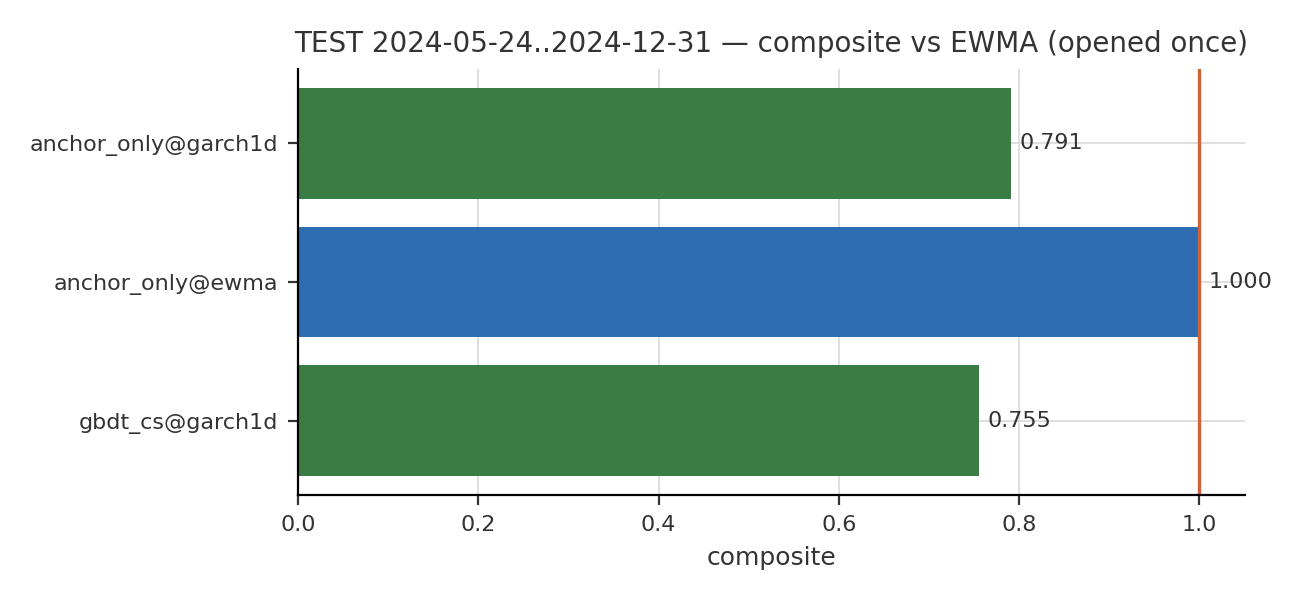
\includegraphics[width=0.55\textwidth]{figures/ml_round2_test.png}
\caption{测试集综合分（参照 EWMA = 1，2024-05-24 至 2024-12-31，开封一次）}
\end{figure}

\subsection{读数：要诚实地归因}
这是本项目第一次在封存测试集上有配置击败 EWMA，但\textbf{大部分收益来自换锚，不是来自机器学习}：GARCH 1 日锚单独就把综合分从 1.000 压到 0.791，ML 在其上再压到 0.755，增量是 0.036 的综合分、约 0.45 美元的 MAE。这一小段 ML 增量在验证集与测试集上方向一致（0.777$\to$0.705，0.791$\to$0.755），测试期 152 个交易日的横截面秩相关每天都为正（均值 0.31）；但标签向前看 252 个交易日而测试期只有 152 天，这些日度读数几乎完全重叠（一阶自相关 0.90），所以这里只说“方向一致”，不给显著性。分工上与最终报告第 7 章一致：随机过程（这里是 GARCH 的条件方差）管水平，ML 管横截面残差。四条保留意见：（1）测试期只有 7 个月、一种市场状态（2024 年下半年，含 8 月初的波动率尖峰）；（2）测试期对 GARCH 锚并不是第一次见面：第 10 周提名它作候选的面板评估覆盖 2019-10 至 2024-12，已经包含本测试期，因此不能拿第 10 周的全样本结果当独立佐证；换锚在测试前的证据是训练期 0.840、验证期 0.777（5.5 节）；ML 增量在更长样本上是否稳定尚未验证；（3）横截面修正基本不移动水平：日均修正只在 $\sigma$ 的 $-1.7\%$ 至 $+0.4\%$ 之间，把修正拆成两部分分别单独使用：只保留水平平移为 0.801，比不修正（0.791）还差；只保留同日内的重排为 0.742，甚至略好于完整修正的 0.755——收益全部来自横截面重排，也因此在所有标的同向出错的日子（例如 2020 年 3 月）它无能为力；（4）行业哑变量带前视（5.5 节）。

\subsection{稳健性诊断（开封之后做，非选择用途）}
以下检查在测试集开封之后进行，不改变上面报告的配置与数字（\texttt{round2\_diagnostics.json}）。
\begin{itemize}
  \item \textbf{行业哑变量的前视}：行业取自当前成分股表，面板里 52 只、7.8\% 的行记为 Unknown：按成分区间核对，其中 51 只后来被移出指数（不少在 2025--2026 年，对面板里任何一天都是未来信息），剩下 1 只是 JPM——它仍在指数中，只是证券表里缺行业字段而被误记。所以 Unknown 基本上编码了“将来会被移出指数”。去掉全部行业哑变量重跑：验证集仍选 GARCH 1 日锚 + GBDT（0.703），测试集 0.741（MAE 7.77），不差于报告值 0.755。报告的结果没有被这项前视抬高；第 12 周接入工具时不使用行业哑变量。
  \item \textbf{换锚的测试前证据}：GARCH 1 日锚相对 EWMA 的综合分，训练期 0.840、验证期 0.777、测试期 0.791。
  \item \textbf{点时守卫}：把原始数据截断在 2024-05-23 重算，截断日之前的特征、EWMA 与 GARCH 锚逐位不变（抽查 JPM、AAPL、XOM）；每个 walk-forward 区块的训练标签窗口都在区块开始前结束。
\end{itemize}

\subsection{SHAP}
测试期 GBDT 的横截面修正由短期已实现波动率（21 日）主导，其次是 252 日与 63 日已实现波动率、当日收益、股息率；行业哑变量的贡献一个数量级更小。解释是干净的：同一天里，近期已实现波动率相对同行更高的标的，其未来一年波动率相对锚更可能向下回复。

\section{理论线 B：隐含波动率锚（JPM，仅本机）}

最终报告第 7 章把“隐含波动率曲面残差”列为 enhancement 首选路线，障碍是个股期权数据。本周用学校 WRDS 账号下的 OptionMetrics 波动率曲面取 JPM 365 天 50-delta 隐含波动率（看涨看跌均值），按许可\textbf{仅在本机作研究检验}，提取文件已加入 git 忽略，不进工具与交付物。在第 4 周 JPM oracle 面板（1293 个交易日，2019-10 至 2024-12）上：

\begin{center}\small
\begin{tabular}{lrrrr}
\toprule
锚 & MAE(\$) & Bias & $R^2$ & 综合分 \\
\midrule
EWMA（参照） & 9.51 & $-1.36$ & $-1.12$ & 1.000 \\
252 日已实现 & 10.31 & $+0.50$ & $-1.12$ & 0.957 \\
\textbf{隐含波动率 365 天} & \textbf{5.90} & $-1.42$ & \textbf{0.10} & \textbf{0.710} \\
\bottomrule
\end{tabular}
\end{center}

表面上 $\ln(\sigma_{iv}/\sigma_{EWMA})$ 与 $\ln(\sigma_{oracle}/\sigma_{EWMA})$ 的相关系数是 0.78，但这是\textbf{机械相关}：两边都含 $-\ln\sigma_{EWMA}$。把隐含波动率换成一个常数，相关系数反而是 0.83。加入隐含波动率对这个比值几乎没有增量解释力（$R^2$ 从 0.688 到 0.689），它与事后真值的时序相关只有 0.04。所以它胜出靠的不是择时，而是\textbf{平稳}：三者的全期均值几乎相同（隐含 26.4\%、EWMA 27.4\%、事后真值 27.3\%），差别在波动幅度——EWMA 的标准差 16.2 个百分点，接近事后真值（8.8）的两倍，隐含波动率只有 4.9，基本停在长期水平附近、不追逐已实现的尖峰。作为诊断，一个取隐含波动率全样本均值的常数锚（用到了全样本，不可部署）综合分 0.532；当时可得的常数型锚（252 日已实现波动率的扩张均值）则是 1.346，输给 EWMA。与 GARCH 锚放在同一窗口比较（GARCH 需要 750 个观测，重叠期为 2020-12 起的 1011 天）：隐含波动率综合分 0.597，GARCH 1 年锚 0.804、GARCH 1 日锚 0.852；但按 MAE，隐含波动率与 GARCH 1 年锚持平（4.20 对 4.18）——后者同样是一条平稳的长期水平线。因此隐含波动率提供的是一个当时可得、平稳且位置合适的水平——这本身是有用的信息——但本检验不能说明它能预测波动率的时变。它对本项目的工具不可用（许可与数据源），只作为方向性证据写进结项报告。

\begin{figure}[H]
\centering
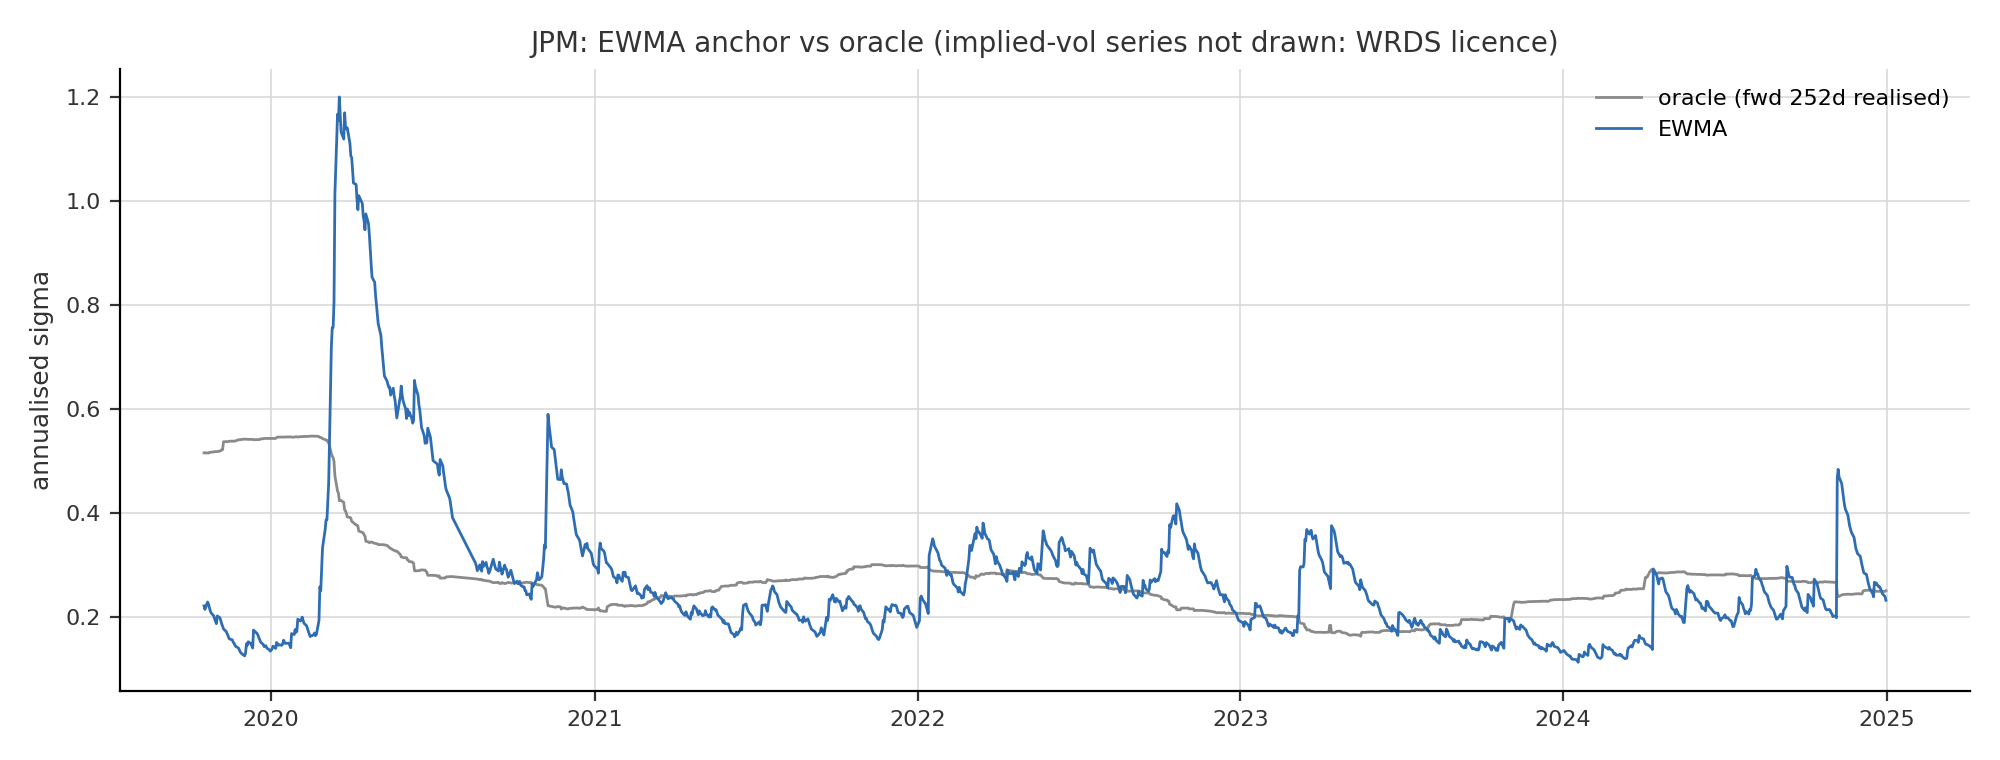
\includegraphics[width=0.80\textwidth]{figures/iv_anchor_jpm.png}
\caption{JPM：EWMA（蓝）围绕事后真值（灰）大起大落；隐含波动率序列按 WRDS 许可不绘出，其均值与标准差见正文}
\end{figure}

\section{对工具的含义与第 12 周}

本周的结果给了第 12 周一个明确的工程决定：把工具的主定价锚从 EWMA 换成 GARCH 1 日预测（训练期、验证期、测试期综合分 0.840 / 0.777 / 0.791，三个窗口都优于 EWMA），并把横截面 GBDT 修正作为面板范围内的 ML 参考价（验证与测试方向一致，测试集 0.755）——符合“只在验证过的范围内展示”的原则。第 12 周：实施换锚（GARCH 参数每 21 日重估、逐票存状态）、把 \texttt{ML\_SCOPE} 扩到面板成员（不使用行业哑变量）、复测全部审计与性能表、写结项报告。

\end{document}
